\section{Indoor localization}
\label{subseq:indoor}

\subsection{Competitors}
Indoor localisation error on 7 scenes~\citep{Shotton2013} dataset are presented in table~\ref{tab:7_scenes}. We compare our proposal with Relocnet~\citep{Purkait2018} and Posenet~\citep{Kendall2017} trained with a geometric-aware loss. At first glance, we find that the initial pose estimation with image retrieval produces decent results (first two columns), while the network used to produce the global image descriptor has not been trained to this particular task. After applying our PnlP pose refinement, the model trained in a fully supervised manner produces the most precise localisation among the presented methods. 

\subsection{Results}
\begin{table}
\centering

\begin{footnotesize}
\renewcommand{\arraystretch}{1.0}
\newcolumntype{Y}{>{\centering\arraybackslash}X}
\begin{tabular}{c l | c c | c c | c c }
					&		&	\multicolumn{2}{c|}{\textit{Image retrieval}} & \multicolumn{2}{c|}{PnlP refinement} & Relocnet & Posenet  \\
	\multicolumn{2}{c|}{Scene} 	&	 \purple{FC-sup.}	  & \blue{FC-unsup.} & \purple{FC-sup.}	& \blue{FC-unsup.}  & \citep{Balntas2018} & \citep{Kendall2017} \\
	\hline	
\multirow{7}{*}{\rotatebox{90}{7-Scenes~\citep{Shotton2013}}}
&		Chess 	&  \purple{\textit{0.29/13.0}} 	& \blue{\textit{0.34/15.4}}	& \textbf{\purple{0.07/2.7}} & \blue{0.13/4.7} & 0.12/4.1 & 0.13/4.5	\\
&		Fire	&  \purple{\textit{0.40/15.5}}	& \blue{\textit{0.48/19.3}}	& \textbf{\purple{0.07/3.2}} & \blue{0.22/8.2} & 0.26/10.4 &	0.27/11.3	\\
&		Heads	&  \purple{\textit{0.28/20.5}}  & \blue{\textit{0.25/17.9}}	& \textbf{\purple{0.05/3.9}} & \blue{0.15/10.5} & 0.14/10.5 & 0.17/13.0		\\
&		Office  &  \purple{\textit{0.38/13.0}}  & \blue{\textit{0.50/16.1}}	& \textbf{\purple{0.09/2.9}} & \blue{0.23/6.3} & 0.18/5.3 & 0.19/5.6		\\
&		Pumpkin &  \purple{\textit{0.43/13.1}}	& \blue{\textit{0.54/15.0}}	& \textbf{\purple{0.13/3.6}} & \blue{0.29/7.1} & 0.26/4.2 & 0.26/4.8		\\
&		Kitchen &  \purple{\textit{0.23/9.5}}   & \blue{\textit{0.26/10.5}}	& \textbf{\purple{0.05/2.0}} & \blue{0.12/3.3} & 0.23/5.1 & 0.23/5.4		\\
&		Stairs  &  \purple{\textit{0.46/14.9}}	& \blue{\textit{0.49/15.5}}	& \purple{0.40/9.2} & \blue{0.48/12.2} & \textbf{0.28/7.5} & 0.35/12.4	\\[1pt]
\hline
\multirow{12}{*}{\rotatebox{90}{12-Scenes~\citep{Valentin2016}}}
& Apt1-kitchen 	& \purple{\textit{0.12/7.7}} & \blue{\textit{0.14/9.2}} & \purple{\textbf{0.09/4.1}} & \blue{0.14/5.0} & - & - \\
& Apt1-living 	& \purple{\textit{0.12/6.8}} & \blue{\textit{0.13/6.7}} & \purple{\textbf{0.08/2.9}} & \blue{0.10/3.3} & - & - \\
& Apt2-kitchen 	& \purple{\textit{\textbf{0.10}/6.5}} & \blue{\textit{\textbf{0.10}/6.6}} & \purple{\textbf{0.10/3.7}} & \blue{\textbf{0.10}/3.9} & - & - \\
& Apt2-living 	& \purple{\textit{0.11/5.6}} & \blue{\textit{0.13/7.3}} & \purple{\textbf{0.10}/4.7} & \blue{0.11/\textbf{3.7}} & - & - \\
& Apt2-bed 		& \purple{\textit{0.13/7.0}} & \blue{\textit{\textbf{0.12}/7.1}} & \purple{\textbf{0.12}/5.7} & \blue{\underline{0.15}/\textbf{5.0}} & - & - \\
& Apt2-luke 	& \purple{\textit{0.15/7.2}} & \blue{\textit{0.16/7.8}} & \purple{\textbf{0.14}/5.5} & \blue{\textbf{0.14/5.3}} & - & - \\
& Office 5a	    & \purple{\textit{0.12/5.3}} & \blue{\textit{0.13/6.3}} & \purple{\textbf{0.09/3.6}} & \blue{\underline{0.14}/4.6} & - & - \\
& Office 5b 	& \purple{\textit{0.15/7.2}} & \blue{\textit{0.18/6.7}} & \purple{\textbf{0.10/4.7}} & \blue{0.14/5.0} & - & - \\
& Lounge	 	& \purple{\textit{0.16/7.1}} & \blue{\textit{0.19/8.3}} & \purple{\textbf{0.10/3.5}} & \blue{0.13/4.7} & - & - \\
& Manolis	 	& \purple{\textit{0.13/6.3}} & \blue{\textit{0.15/7.8}} & \purple{\textbf{0.09/3.7}} & \blue{0.12/4.5} & - & - \\
& Gates362	 	& \purple{\textit{0.13/5.9}} & \blue{\textit{0.14/6.5}} & \purple{\textbf{0.10}/4.7} & \blue{0.11/\textbf{3.9}} & - & - \\
& Gates381 		& \purple{\textit{0.15/7.7}} & \blue{\textit{0.16/9.0}} & \purple{\textbf{0.11/4.4}} & \blue{0.13/5.1} & - & - \\
\end{tabular}
\end{footnotesize}

\caption{\label{tab:7_scenes} Results on the \textbf{7 scenes}~\citep{Shotton2013} and \textbf{12 scenes}~\citep{Valentin2016} indoor datasets, we report median position/orientation error in meters/degree. We compare the first pose estimation (im. retrieval, \textit{in italics}) and, the final image localisation (PnlP) of our method and two state-of-the-art approaches. Best localisation results are shown in \textbf{bold} and \underline{underligned} numbers show failure cases when the pose refinement increases the initial pose error. Sup. (\purple{in purple}) and unsup. (\blue{in blue}) stand for supervised, respectively unsupervised, depth from monocular training. Table best viewed in color.}


\end{table}
\begin{figure}
    \centering

	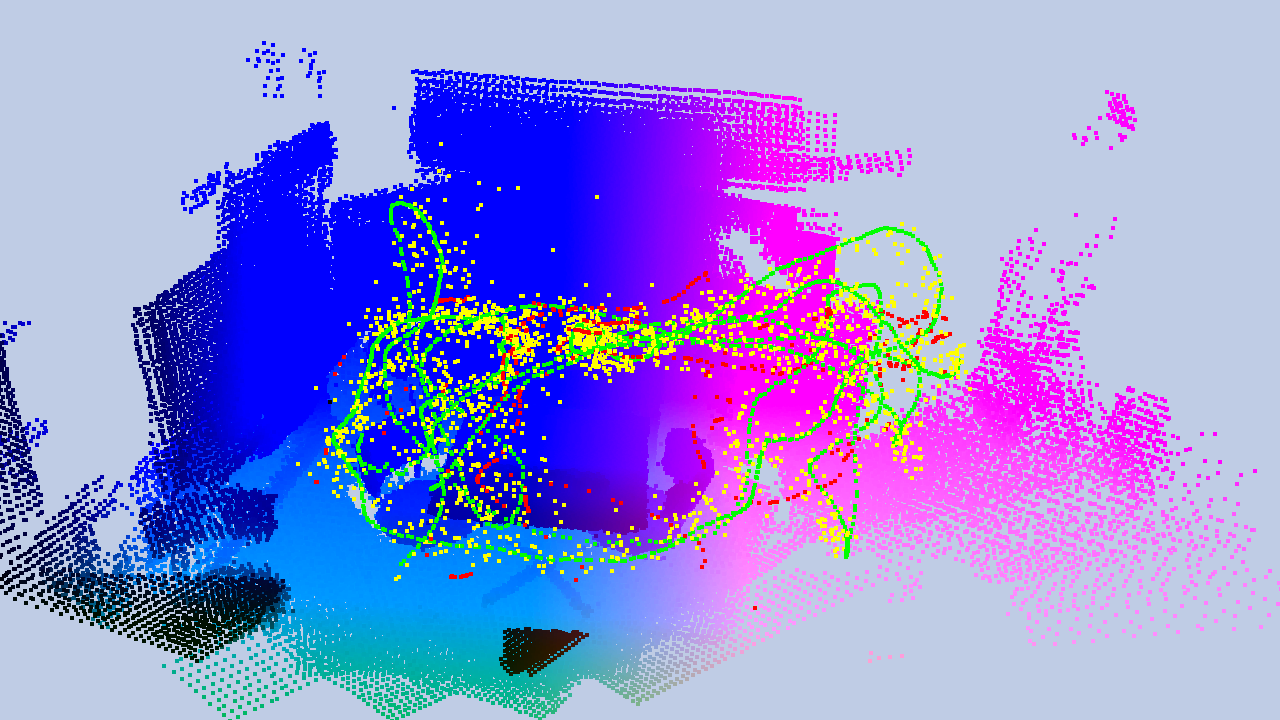
\includegraphics[width=\linewidth]{results/models/chess}
	
	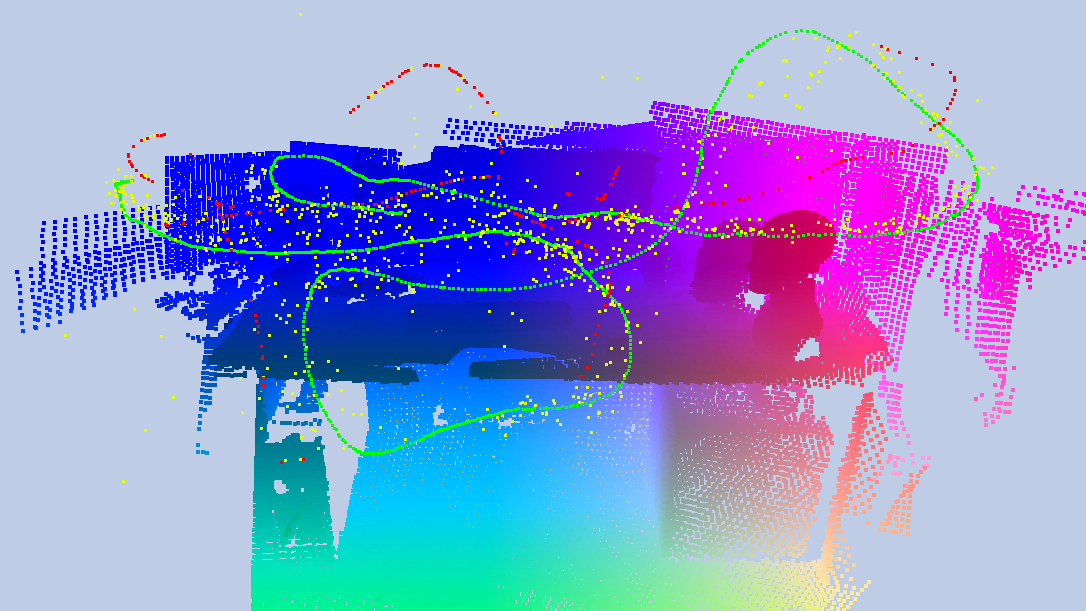
\includegraphics[width=\linewidth]{results/models/heads}
	
	\caption[]{\label{fig:res_visualization2} .}
	
\end{figure}

\begin{figure}
	\centering
	
	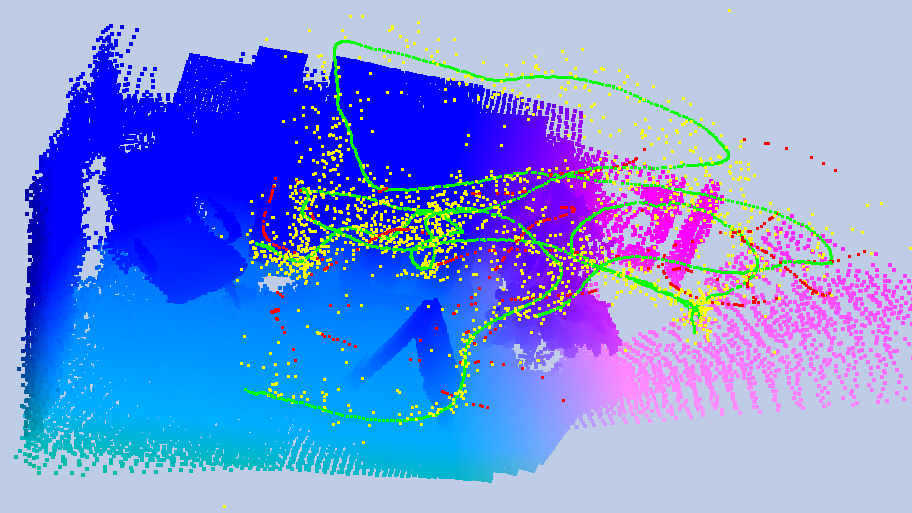
\includegraphics[width=\linewidth]{results/models/fire}
	
	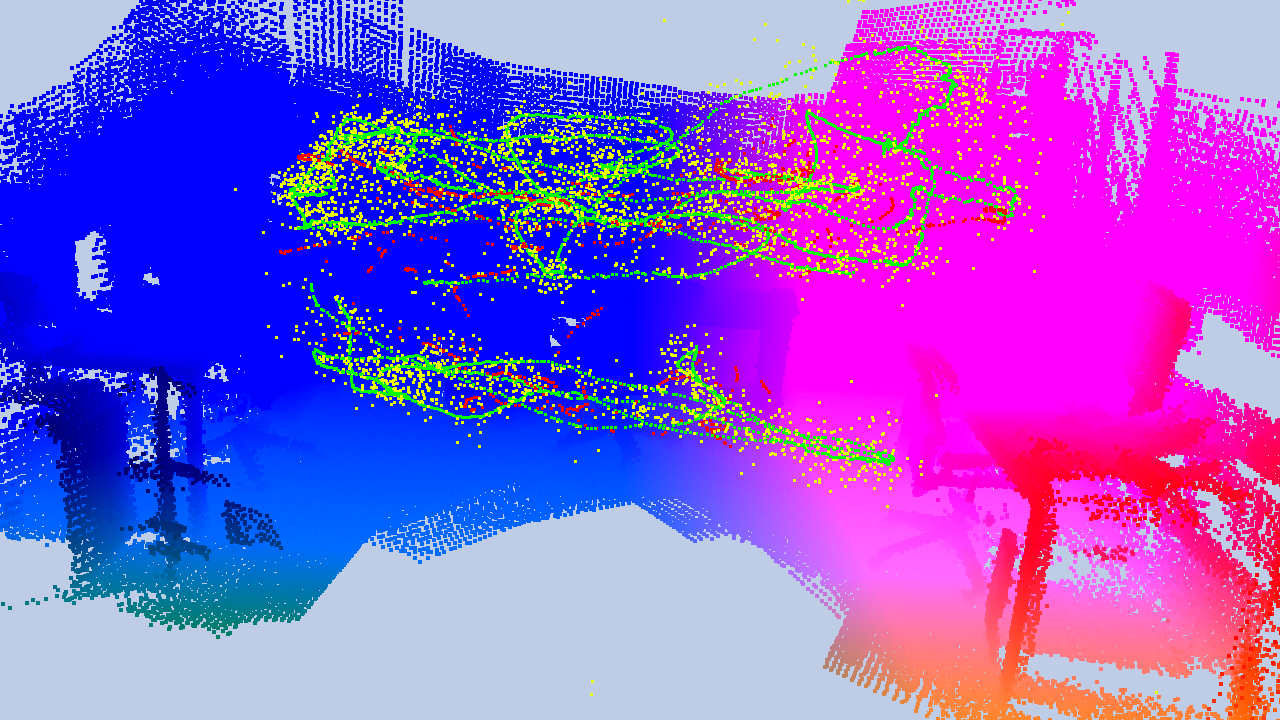
\includegraphics[width=\linewidth]{results/models/office}

	
	\caption[]{\label{fig:res_visualization1} .}
	
\end{figure}
For the unsupervised setting, we found that FC and C+LSTM architectures perform equivalently on the indoor dataset, thus we present only results of the FC architecture. We observe an average relative improvement of $\times$2.8/$\times$3.5, respectively $\times$1.8/$\times$2.1, for the supervised, respectively unsupervised, model in position/rotation from initial to PnlP refined pose. Compared to Posenet~\citep{Kendall2017} our unsupervised model perform equivalently, while using the same trained network for all the 7 scenes, compared to one network by scene for Posenet. Our proposal clearly outperforms Relocnet~\citep{Balntas2018} in a supervised setting, while producing comparable localisation for the model trained in an unsupervised manner. It is important to remind that Relocnet relies on two different networks: one trained especially to produce discriminative global image descriptors for CBIR and the second to estimate the relative pose between two images. Our method is lighter as it uses a single network and do not uses specific training for the task of global image description. We observe a failure case of our method for the scene stairs due to a poor initial pose estimation. This scene contains repetitive visual patterns that may confuse the CBIR localisation.

\subsection{Generalisation} 
\begin{figure}
    \centering

	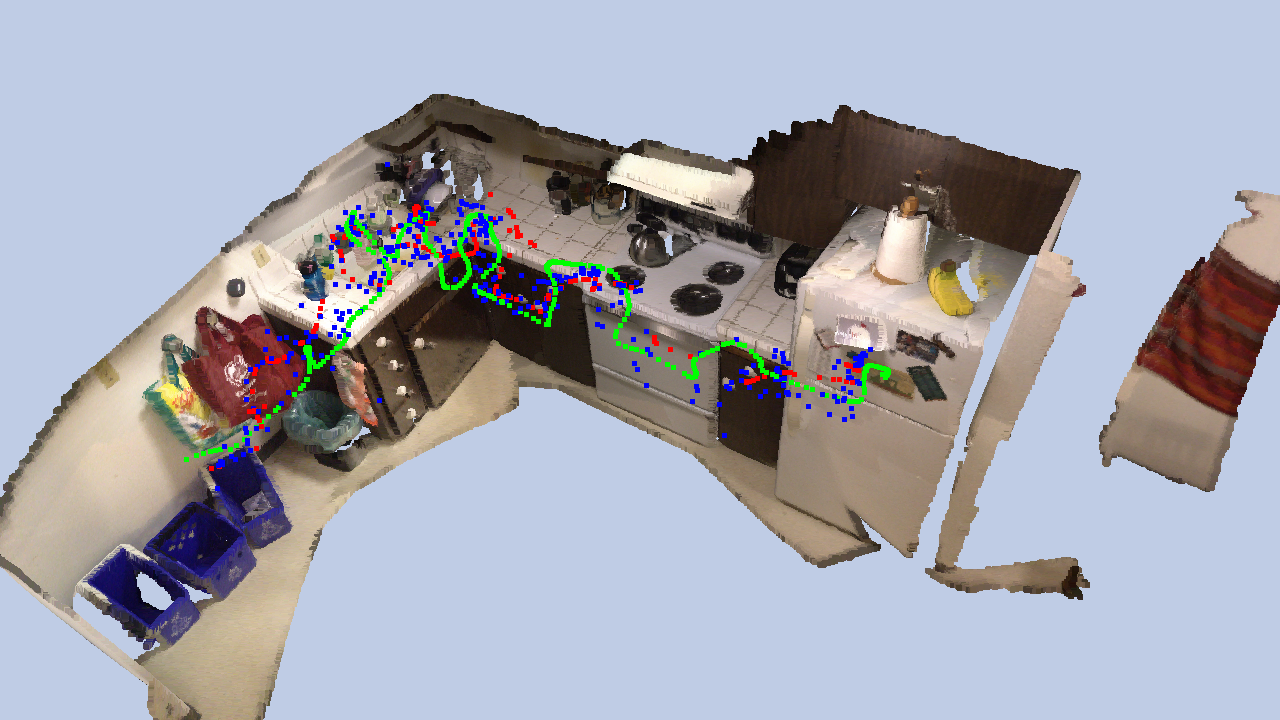
\includegraphics[width=\linewidth]{results/models/kitchen}
	
	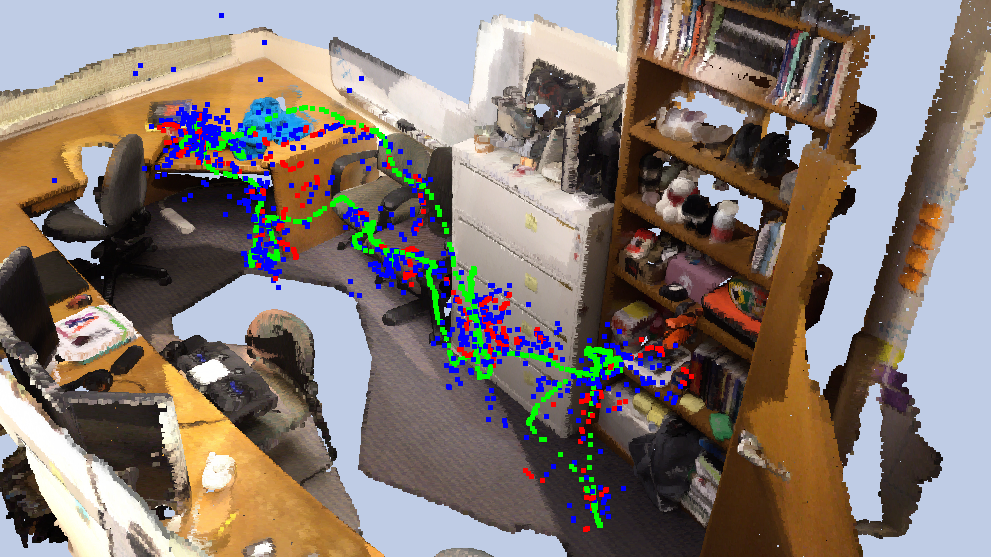
\includegraphics[width=\linewidth]{results/models/manolis}
	
	\caption[]{\label{fig:res_visualization_gene} .}
	
\end{figure}
We also report on table~\ref{tab:7_scenes} localization error on 8 scenes of the 12 Scenes dataset~\citep{Valentin2016}. For these experiments, we use the same network as mentioned earlier, trained on 7 Scenes dataset~\citep{Shotton2013}. We observe an average relative improvement of $\times$1.2/$\times$1.5, respectively $\times$1.1/$\times$1.6, for the supervised, respectively unsupervised, model in position/rotation from initial to refined pose. Even though the pose refinement is not as effective as previously, it shows that our system can be used on completely new indoor environments. We also demonstrate, in figure~\ref{fig:depth_map_indoor}, the generalization capability of our method through the depth maps produced by our networks, from images taken on both known and unknown scenes. We notice that the poor localization performance on the Apt2-bed scenes is closely related to the poor generated depth map on this scene (see figure~\ref{fig:depth_map_indoor}, two last columns).
